\def\longueurVecteurs{1.75}
\def\interSpace{0.5}
\def\interSpaceY{2}

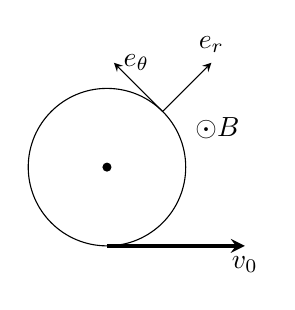
\begin{tikzpicture}
  \tikzstyle{fleche}=[->,>=stealth];
  %\draw [fleche] (0,0) -- (\longueurVecteurs,0) node [above] {$\vv{e_r}$};
  %\draw [fleche] (0,0) -- (0,\longueurVecteurs) node [right] {$\vv{e_\theta}$}; 
  \draw [fleche] (0.707,0.707) -- +(45:\longueurVecteurs/2) node [above] {$\vv{e_r}$};
  \draw [fleche] (0.707,0.707) -- +(135:\longueurVecteurs/2)  node [right] {$\vv{e_\theta}$};
  \draw [fleche, very thick,\JRLblue] (0,-1) -- (\longueurVecteurs,-1) node [below] {$\vv{v}_0$};
  %\draw [fleche] (\longueurVecteurs/2,0) arc (0:45:\longueurVecteurs/2) node [midway,right] {$\alpha$}; 
  \draw (1,0.5) node [right] {$\odot \vv{B}$};
  %\draw (0,0) node[below left]{$\ptO$};
  \draw (0,0) circle (1);
  \filldraw (0,0) circle (0.05);
  \draw (0,0) node [above] {$\ptC$};
\end{tikzpicture}
